\section{Comparison with Real Data}
\label{sec:comparison}

To evaluate the precision of the methods used for the assignment, the models were compared with real data of the payload SDO, NORAD Catalogue Number 36395, from \cite{space_track} \cite{n2yo}. This choice was motivated because the payload’s orbit is similar to the nominal orbit of the assignment. The altitude of the orbit is also in the GSO region, which means the J2 effect and Moon disturbances are very prominent in the region. It is also important to note that a payload will correct its orbit using active propulsion. As the numerical model does not consider this kind of manoeuvres, a worse coincidence between results is expected. To compute the orbit propagation, the initial orbital elements were those collected from Space-Track at the initial time, shown on the table. To propagate the orbit, Gauss’ planetary equations in RSW frame were solved numerically using ode113. A low-pass filter of frequency $0.4949  day^{-1}$ was used to get the mean value every two orbits, considering the initial period. Filtering was done using \( N = \lceil \frac{T_{cut}}{\Delta t} \rceil \). \( T_{cut} \) is the period of the oscillation to discard and \( \Delta t \) is the time step of the propagation. 

%cite: space-track.org
%cite: https://www.n2yo.com/satellite/?s=36395

\begin{table}[ht]
	\centering
	\label{tab:keplerian_elements_2}
	\begin{tabular}{|c|c|c|c|c|c|}
		\hline
		a [km] & e [-] & i [$\deg$] & $\Omega$ [$\deg$] & $\omega$ [$\deg$] & $h_p$ [km] \\
		\hline
		42165.38456 & 0.000069 & 27.833 & 169.5864 & 245.7244 & 35783.9 \\
		\hline
	\end{tabular}
	\caption{Keplerian elements of orbit}
\end{table}

From the figures below, it can be observed that the numerical approach is capable of estimating the orbit with good reliability as the trends of both results are very similar. The differences seen on each plot were expected, as only J2 and Moon perturbations were taken into account for the numerical model. There’s a great difference in the short-term behaviour between numerical simulation and the real data. As the numerical simulation can generate data for any time interval, it can evaluate the short-term oscillations, while the real data is measured with a broader list of other elements that can change the values of the Keplerian data.

\newcommand{\n}{0.7}

\begin{figure}[H]
	\begin{minipage}{0.48\linewidth}
		\centering
		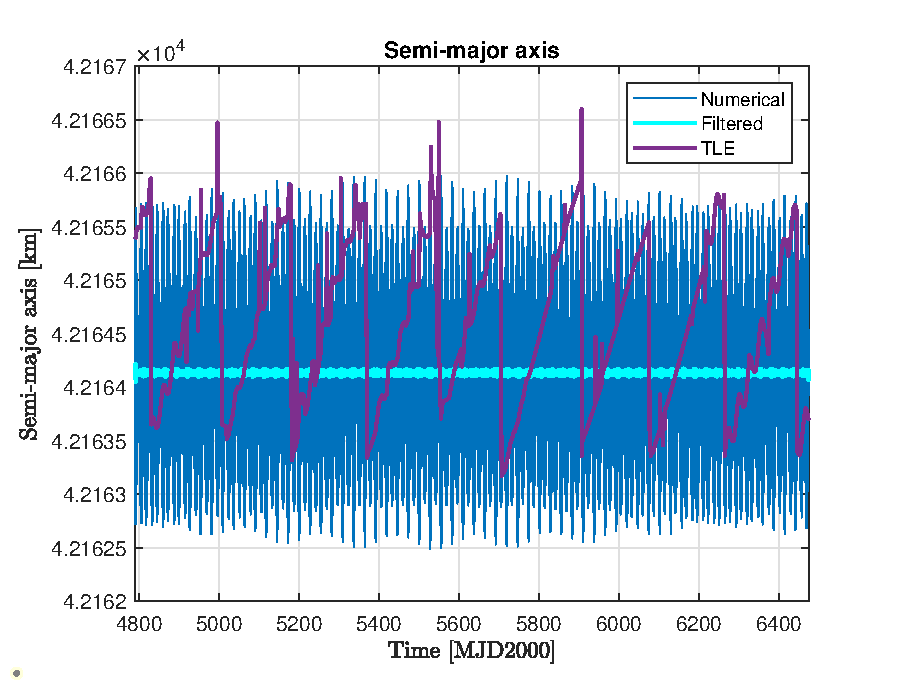
\includegraphics[width=\n\linewidth]{a_TLE.eps}
	\end{minipage}\hfill
	\begin{minipage}{0.48\linewidth}
		\centering
		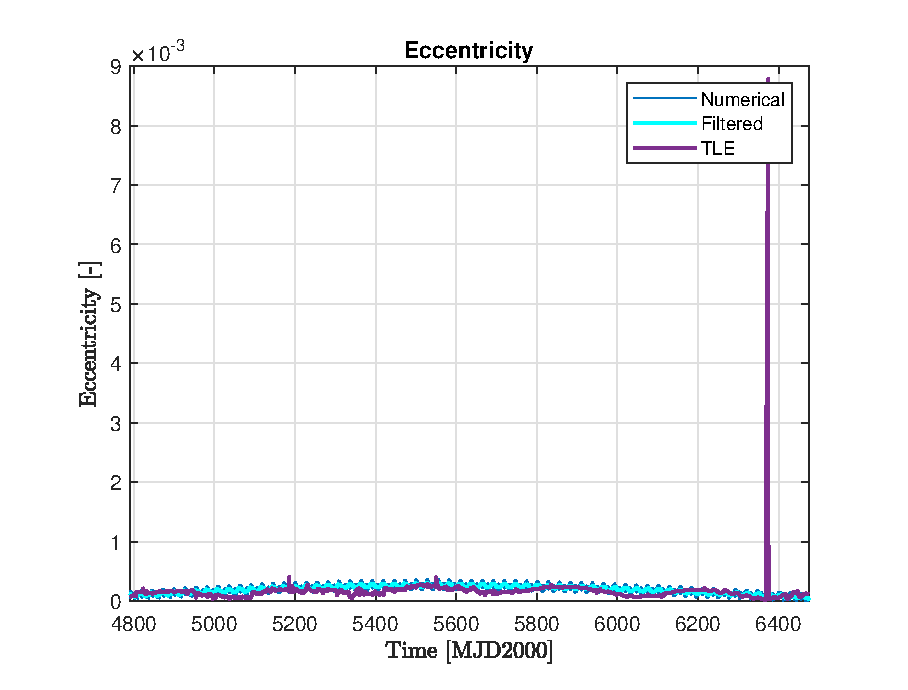
\includegraphics[width=\n\linewidth]{e_TLE.eps}
	\end{minipage}
	\vfill
	\begin{minipage}{0.48\linewidth}
		\centering
		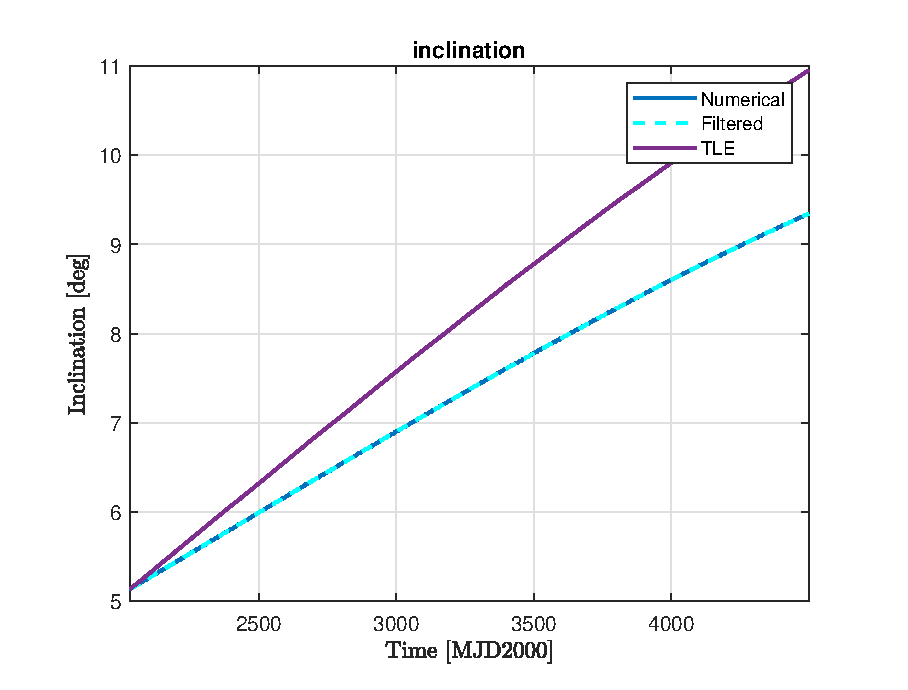
\includegraphics[width=\n\linewidth]{i_TLE.eps}
	\end{minipage}\hfill
	\begin{minipage}{0.48\linewidth}
		\centering
		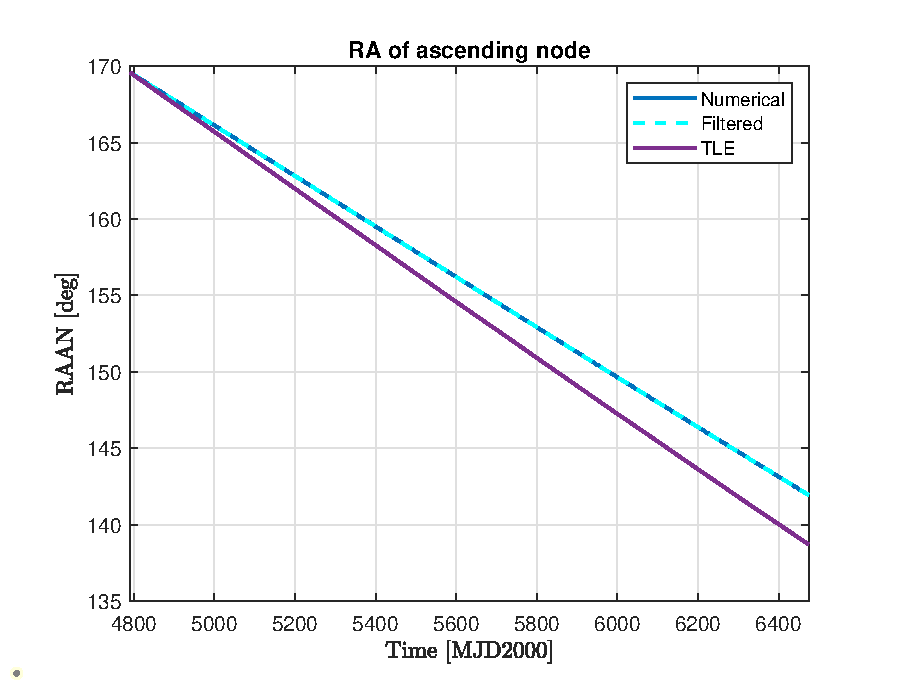
\includegraphics[width=\n\linewidth]{RAAN_TLE.eps}
	\end{minipage}
	\vfill
	\begin{minipage}{0.48\linewidth}
		\centering
		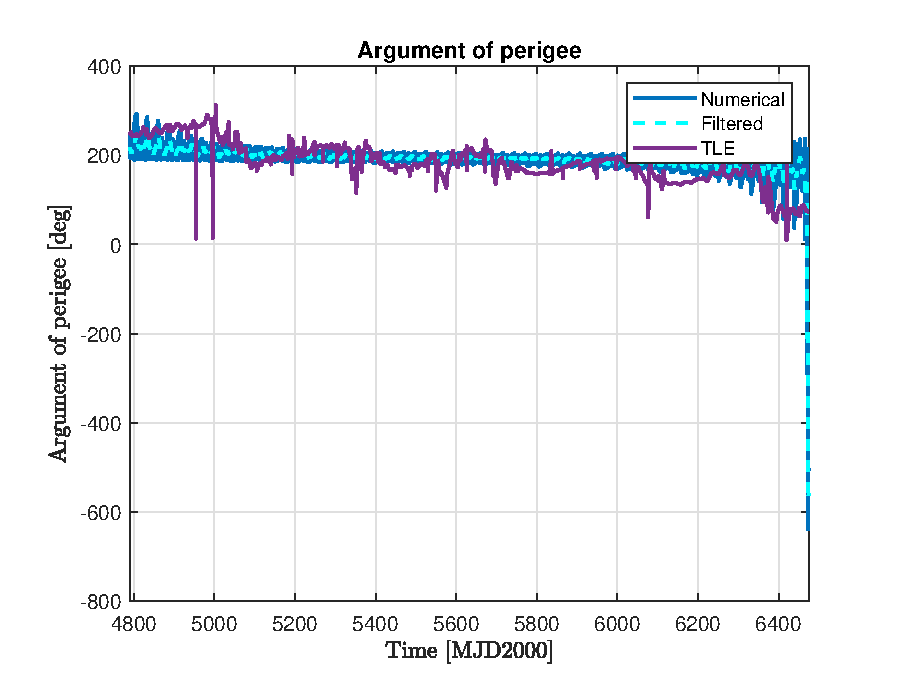
\includegraphics[width=\n\linewidth]{w_TLE.eps}
	\end{minipage}\hfill
	\begin{minipage}{0.48\linewidth}
		\centering
		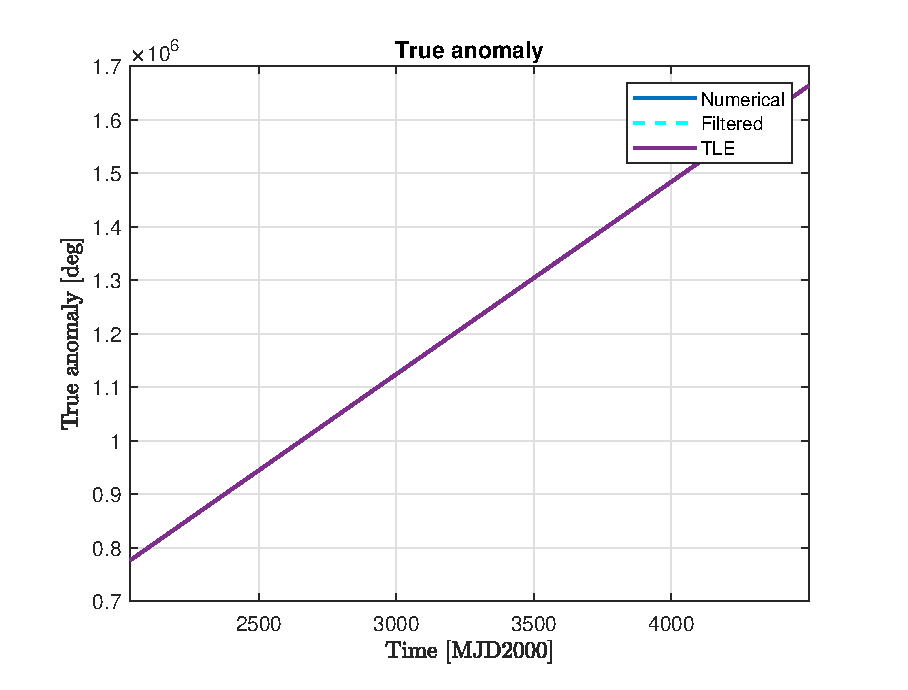
\includegraphics[width=\n\linewidth]{TA_TLE.eps}
	\end{minipage}
	\caption{Numerical, filtered and TLE data}
	\label{fig:comparison_figures}
\end{figure}